% Created 2021-04-25 Sun 00:05
% Intended LaTeX compiler: pdflatex
\documentclass[9pt, b5paper]{article}
\usepackage[UTF8]{ctex}
\usepackage{fontspec}
\usepackage{graphicx}
\usepackage{xcolor}
\usepackage{multirow}
\usepackage{multicol}
\usepackage{float}
\usepackage{textcomp}
\usepackage{geometry}
\geometry{left=1.2cm,right=1.2cm,top=1.5cm,bottom=1.2cm}
\usepackage{algorithm}
\usepackage{algorithmic}
\usepackage{latexsym}
\usepackage{natbib}
\usepackage{listings}
\usepackage{minted}
\usepackage[xetex,colorlinks=true,CJKbookmarks=true,linkcolor=blue,urlcolor=blue,menucolor=blue]{hyperref}
\author{deepwaterooo}
\date{\today}
\title{成长的故事——我和舅舅}
\hypersetup{
 pdfauthor={deepwaterooo},
 pdftitle={成长的故事——我和舅舅},
 pdfkeywords={},
 pdfsubject={},
 pdfcreator={Emacs 27.1 (Org mode 9.3)}, 
 pdflang={English}}
\begin{document}

\maketitle
\tableofcontents


\section{行走在《计算机》专业的大道上(2)——第一学期}
\label{sec:org8910421}

先前所有的基础再列一遍

\begin{center}

\includegraphics[width=.9\linewidth]{./pic/backups_plans_20210424_203000.png}
\end{center}

绝对不可以跳过CS121这门最基础的编程课

\begin{center}

\includegraphics[width=.9\linewidth]{./pic/backups_plans_20210424_203059.png}
\end{center}

选课的情况:换课,不要故意挫败自己


\begin{center}

\includegraphics[width=.9\linewidth]{./pic/backups_plans_20210424_203308.png}
\end{center}

最开始的学习状态:弱弱还是怕的!

\begin{center}

\includegraphics[width=.9\linewidth]{./pic/backups_plans_20210424_203440.png}
\end{center}

\begin{center}

\includegraphics[width=.9\linewidth]{./pic/backups_plans_20210424_203454.png}
\end{center}

所遭受到的莫名其妙的、不名所以的打击:

\begin{center}

\includegraphics[width=.9\linewidth]{./pic/backups_plans_20210424_203548.png}
\end{center}

\begin{center}

\includegraphics[width=.9\linewidth]{./pic/backups_plans_20210424_203612.png}
\end{center}

当年的小弱弱呀(2014年夏天写的、回忆2012年9月份课堂),这段写得好touchy,读起来惹得我好心疼当年的自己!

\begin{center}

\includegraphics[width=.9\linewidth]{./pic/backups_plans_20210424_210229.png}
\end{center}

写自己学习上的崩溃瞬间:硕士研空生代课老师——系里学历最低的代课老师,他就是系里打压学生时专业负责打扫卫生的,接下来所有这类脏活他全干

\begin{center}

\includegraphics[width=.9\linewidth]{./pic/backups_plans_20210424_155915.png}
\end{center}

\begin{center}

\includegraphics[width=.9\linewidth]{./pic/backups_plans_20210424_160112.png}
\end{center}

写女生公主


\begin{center}

\includegraphics[width=.9\linewidth]{./pic/backups_plans_20210424_203858.png}
\end{center}

怎么感觉老师讲课的内容就是听不懂,不知道老师究竟在说什么呢?

再举几个例子试试看:其它老师的代课风格???

\begin{center}

\includegraphics[width=.9\linewidth]{./pic/backups_plans_20210424_204032.png}
\end{center}

在老师的示意下,回答了问题的自己的状态:带着点儿自信

\begin{center}

\includegraphics[width=.9\linewidth]{./pic/backups_plans_20210424_204405.png}
\end{center}

老师的态度又如何呢?
再回想一下:应该这样吗?我是否应该再稍微大胆一点儿呢?
老师是在故意想要掩藏我的光茫吗?为什么呢?为了来年夏天的实习吗?

写自己与代课老师的君子协议:没必要

TicTacToe:

\begin{center}

\includegraphics[width=.9\linewidth]{./pic/backups_plans_20210424_205732.png}
\end{center}

\begin{center}

\includegraphics[width=.9\linewidth]{./pic/backups_plans_20210424_205104.png}
\end{center}

\begin{center}

\includegraphics[width=.9\linewidth]{./pic/backups_plans_20210424_205605.png}
\end{center}

写自己的爸爸泪崩:亲情的温暖

食堂虚脱:没有人情,累死你也要把你放到最后一个去吃饭

对表哥的深深思念

\begin{center}

\includegraphics[width=.9\linewidth]{./pic/backups_plans_20210424_205932.png}
\end{center}

CS121想给我成绩C:没有公正的系统、每门课都会打压成绩

\begin{center}

\includegraphics[width=.9\linewidth]{./pic/backups_plans_20210424_210025.png}
\end{center}

其实我应该是可以拿A的,可是为什么没有争取呢?

\begin{center}

\includegraphics[width=.9\linewidth]{./pic/backups_plans_20210424_210204.png}
\end{center}

\begin{center}
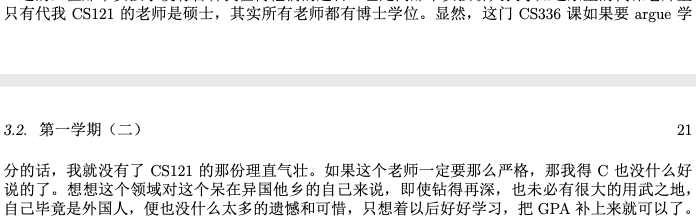
\includegraphics[width=.9\linewidth]{./pic/backups_plans_20210424_210328.png}
\end{center}

另一门课的情况CS336:

我的室友呢?

\begin{center}

\includegraphics[width=.9\linewidth]{./pic/backups_plans_20210424_210542.png}
\end{center}

政治庇护:最好不要

\begin{center}

\includegraphics[width=.9\linewidth]{./pic/backups_plans_20210424_210639.png}
\end{center}

朋友的情况:一个在食堂里认识的中国女生,以及她的结果,可以把她想要的爱情也写一下,一个台湾男生

\begin{center}

\includegraphics[width=.9\linewidth]{./pic/backups_plans_20210424_212545.png}
\end{center}

\begin{center}

\includegraphics[width=.9\linewidth]{./pic/backups_plans_20210424_220817.png}
\end{center}

早上

\begin{center}

\includegraphics[width=.9\linewidth]{./pic/backups_plans_20210424_212910.png}
\end{center}

十二月的一次

\begin{center}

\includegraphics[width=.9\linewidth]{./pic/backups_plans_20210424_213118.png}
\end{center}

\begin{center}

\includegraphics[width=.9\linewidth]{./pic/backups_plans_20210424_213150.png}
\end{center}

第二学期的病情

身体上的不适:两次生病的情况

\begin{center}

\includegraphics[width=.9\linewidth]{./pic/backups_plans_20210424_095434.png}
\end{center}

有一次食堂里虚脱了:写食堂里工作人员的无情

12月考完后去看医生

\section{行走在《计算机》专业的大道上(3)——第二学期}
\label{sec:org9ca62ad}

\begin{center}

\includegraphics[width=.9\linewidth]{./pic/backups_plans_20210424_213617.png}
\end{center}

可以听到小弱弱的弱弱的气息,那个当年脆弱而无助的孩子,摸摸。


\begin{center}

\includegraphics[width=.9\linewidth]{./pic/backups_plans_20210424_213746.png}
\end{center}


\begin{center}

\includegraphics[width=.9\linewidth]{./pic/backups_plans_20210424_213816.png}
\end{center}


\begin{center}

\includegraphics[width=.9\linewidth]{./pic/backups_plans_20210424_215400.png}
\end{center}

\begin{center}

\includegraphics[width=.9\linewidth]{./pic/backups_plans_20210424_215822.png}
\end{center}

CS570

\begin{center}

\includegraphics[width=.9\linewidth]{./pic/backups_plans_20210424_214439.png}
\end{center}

每每读到小弱弱当年喘着虚弱的气息般的描述,都感到辛酸、心疼——心疼当年那个朴实的孩子!

\begin{center}

\includegraphics[width=.9\linewidth]{./pic/backups_plans_20210424_214802.png}
\end{center}

\begin{center}

\includegraphics[width=.9\linewidth]{./pic/backups_plans_20210424_214908.png}
\end{center}

这是不是又是另一种的执念呢?为什么老师说的话,对你就像过耳东岁般,你就听不进去呢?

RTOS

\begin{center}

\includegraphics[width=.9\linewidth]{./pic/backups_plans_20210424_213859.png}
\end{center}

\begin{center}

\includegraphics[width=.9\linewidth]{./pic/backups_plans_20210424_213910.png}
\end{center}

小弱弱的幼稚心思,当年会做出这样的事情,现在读起来都还觉搞笑、还有点儿小女孩般的幼稚可爱(哈哈)!

\begin{center}

\includegraphics[width=.9\linewidth]{./pic/backups_plans_20210424_213954.png}
\end{center}

\begin{center}

\includegraphics[width=.9\linewidth]{./pic/backups_plans_20210424_214124.png}
\end{center}

经济资助

\begin{center}

\includegraphics[width=.9\linewidth]{./pic/backups_plans_20210424_215120.png}
\end{center}

\begin{center}

\includegraphics[width=.9\linewidth]{./pic/backups_plans_20210424_215147.png}
\end{center}

\begin{center}

\includegraphics[width=.9\linewidth]{./pic/backups_plans_20210424_215618.png}
\end{center}

\begin{center}
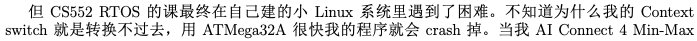
\includegraphics[width=.9\linewidth]{./pic/backups_plans_20210424_215728.png}
\end{center}

\begin{center}

\includegraphics[width=.9\linewidth]{./pic/backups_plans_20210424_215743.png}
\end{center}


\begin{center}

\includegraphics[width=.9\linewidth]{./pic/backups_plans_20210424_220650.png}
\end{center}

食堂打工怎么样呢?

\begin{center}

\includegraphics[width=.9\linewidth]{./pic/backups_plans_20210424_220153.png}
\end{center}

\begin{center}

\includegraphics[width=.9\linewidth]{./pic/backups_plans_20210424_220214.png}
\end{center}

夏天实习

\textbf{备注:}
尘世将就过的婚姻的部分只写了一半,还没写完,可能今天晚时候或者明天才发出来
回到学校的内容一时半会儿还是不知道怎么写怎么立意,先尝试着写这一个学期、或是第一年的学习成长,感觉一下,再去看是否先写夏天实习(感觉这么写更自然一些),还是把计算机专业写完
因为后来情商回来稍高一点儿,很多事情都被如实记载过,一方面我会努力写深一点儿(以事后诸葛亮、过来人的眼光回望那一程风雨兼程),另一方面可能也只能借助谋篇组篇重新组合才能读起来连贯有感觉,所以接下来的内容、绝大部分的内容可能都会被打乱顺序与重新组篇,个别需要时间连贯的除外。
这个先尝试一两篇,感觉一下,看接下来该如何提升写法。

\section{盘旋在校园上空的三大舆论“监控”力量}
\label{sec:org640904e}

2012年秋天,当我怀揣对《计算机》专业的一丝敬畏,我重返校园,去读一个这个专业的硕士学位。

那个曾经盯紧我、实时监控我、发动舆论炒作过我、把我当成他们三大网站自家网红、前后两年(2011、2012)先后给我下放过两次申请H1B工作机会的三大舆论场,现在、接下来的年月里会做些什么呢?

2011年她情商不够,第一次他们过于草率的逼良为娼行为就那么轻易失败了;

一年后,已经被她舅舅电邮件语言警告、并于8月头亲自播打了911、不断反复收到来自她表哥的电子邮件一再拒绝,切断了与她舅舅家、与她那表哥的一切联系,按理说她心目中对她表哥的那点儿动心留恋早该清除干净了吧——如果对也来说真的曾经有过心动的话。可为什么那个生活在、沉溺在她刻舟求剑的梦里总不肯醒来的傻子就那么——那么地傻,傻到连掉到她嘴边的鸭子肥肉(H1B申请工作签证的机会)就那么被她华丽丽地放跑放飞了?

那个白痴,她的情商在哪里?

如果说2012年秋季返校,对我来说是一个新的起点,开启了一场更深层的发挖、探索与成长之旅,那么同期的三大舆论场,也开始了他们对我这个他们紧盯的目标、在统计实习29个月期间所有的重点章节、细节、也发起了一场浩大的舆论反刍、勘测探究之旅——为的是,找到那埋藏在地面之下地底层的煤矿——她的情商、精神状态所在之地?

\begin{center}

\includegraphics[width=.9\linewidth]{./pic/backups_plans_20210424_101221.png}
\end{center}

三大舆论的反刍也是他们在勘探与寻找:这个被他们紧盯着,混在了全部由他们的托儿组成的游山玩水、打羽毛球等队伍中、过着青蛙王子般似水流年的目标,她这些年、这29个月的情商到底在哪里?

我以为,盘旋在校园上空的来自于三大中文的这股舆论监控力量,也是三大所采取的一种寻找、求证与证实他们猎物精神状态的途径与过程。


\begin{center}

\includegraphics[width=.9\linewidth]{./pic/backups_plans_20210424_220444.png}
\end{center}

他们故意炒作说我可以拿奖学金,但是我的学习基础不够。
想要继续共情的炒作培养同理心

\subsection{(一)肯定编程、鼓励学习}
\label{sec:org46f213f}

\begin{center}
\includegraphics[width=.9\linewidth]{./pic/backups_plans_20210424_100901.png}
\end{center}

最先出现的是2012年9月来自于成名——三大的托儿的电话!

这也是一种鼓励:如果给编程序,如果能把这个专业努力学好,将来不愁找不到工作、将来不愁无法生存!所以,还是要努力好好学习。

成名不是计算机专业只读一两年就找到工作不读了吗?当时的自己为什么不曾想起这个?

2011年春天奥克兰的那份工作的女生不是双专业、有计算机学位去做了统计相关的工作,工作机会不是大把大把地往外涌吗?!!!

另一层意思:同样,百尺竿头,更进一步!

\subsection{(二)2011年——职场投放的第一次电梯}
\label{sec:org9b29e46}

\begin{center}
\includegraphics[width=.9\linewidth]{./pic/backups_plans_20210424_205834.png}
\end{center}

接下来他们洗劫、征求状态、掀起的舆论的焦点便是关于2011年春季的那分职场工作——这个白痴一样的猎物,当时到底算是怎么回事儿呢?

\begin{center}
\includegraphics[width=.9\linewidth]{./pic/backups_plans_20210424_093531.png}
\end{center}

那时我也不知道是为什么、学习紧张、没有时间、时间不够,还是那时的自己看不到那时工作中已婚女同事的立场、经历与接下来的工作发展与自己有多深的相关性?

\begin{center}
\includegraphics[width=.9\linewidth]{./pic/backups_plans_20210424_094006.png}
\end{center}

后来刚过去不久,等我真正硅谷红尘游历一番,世事看尽看透,再去回想当年的那些人、那些事,终于还是把那部分不曾觉得重要的部分补充出来。

\begin{center}
\includegraphics[width=.9\linewidth]{./pic/backups_plans_20210424_102201.png}
\end{center}

part I page 127-128这两页中的部分内容。

\begin{center}
\includegraphics[width=.9\linewidth]{./pic/backups_plans_20210424_102322.png}
\end{center}

这些,都是舅舅与表哥曾经给予过他们的确信。

\begin{center}
\includegraphics[width=.9\linewidth]{./pic/backups_plans_20210424_102504.png}
\end{center}

\begin{center}
\includegraphics[width=.9\linewidth]{./pic/backups_plans_20210424_102530.png}
\end{center}

而几个月前五月底,当他们的托儿站出来给我洗脸,相要掐灭我心目中的爱情的时候,她所站过的立场:她总是很理解舅舅和我表哥,但对我各种尖酸刻薄!

以及,在他们确认我亲爱的表哥与我的舅舅、是永远站在他们的立场上,与他们是同一条心的,

\subsection{(三)朋友:寻找探讨其它婚姻对象存在与否、并进行必要铲除?}
\label{sec:org87e69f1}

那么,我的周围的生活圈是否还有其它潜在发展成为爱情、或者简单点儿——将来世俗婚姻对象的存在?

\begin{center}
\includegraphics[width=.9\linewidth]{./pic/backups_plans_20210424_102654.png}
\end{center}

这是更早一点儿时间已经简单澄清过的

\begin{center}
\includegraphics[width=.9\linewidth]{./pic/backups_plans_20210424_134105.png}
\end{center}

后来没有办法,只好把整个过程再写得更为详尽一点儿

\begin{center}
\includegraphics[width=.9\linewidth]{./pic/backups_plans_20210424_113449.png}
\end{center}

\begin{center}
\includegraphics[width=.9\linewidth]{./pic/backups_plans_20210424_102814.png}
\end{center}


\subsection{(四)傻不傻、真傻还是假傻:再炒几件看看、评估一下}
\label{sec:org5ddc024}

就列几件事情吧:

\begin{center}
\includegraphics[width=.9\linewidth]{./pic/backups_plans_20210424_103008.png}
\end{center}

3、9/2013:食堂里的事儿。暂时不在这里写,写进学校里的成长里面

然后他们的托儿自己组织过的饭局的反思

\begin{center}
\includegraphics[width=.9\linewidth]{./pic/backups_plans_20210424_103043.png}
\end{center}

\begin{center}
\includegraphics[width=.9\linewidth]{./pic/backups_plans_20210424_093212.png}
\end{center}

可以肯定,这股舆论的力量来自于三大。因为2010、2011年,我在硅谷建立起来的所谓的朋友圈,实则全都是三大的托儿的存在,包括2011年当时我假装喜欢过与他一起打篮球的男生和那时游山玩水的小伙伴队伍,这是后话。 

\subsection{(五)表哥,还是属于她的吗}
\label{sec:orgc3c2dc2}

\begin{center}
\includegraphics[width=.9\linewidth]{./pic/backups_plans_20210424_133752.png}
\end{center}

炒作当年学统计的我,与学计算机的表哥,他们炒作的方向当然是想要拆开表哥与我这对佳侣(——为的是他们将来要逼良为娼的目的,早折对他们来说早好!)。

\begin{center}
\includegraphics[width=.9\linewidth]{./pic/backups_plans_20210424_133949.png}
\end{center}

加入与我表哥联系的部分

\subsection{(六)网络名誉:继续打造世外天仙}
\label{sec:orgf4ee5e8}

\begin{center}
\includegraphics[width=.9\linewidth]{./pic/backups_plans_20210424_094918.png}
\end{center}

\begin{center}
\includegraphics[width=.9\linewidth]{./pic/backups_plans_20210424_095706.png}
\end{center}

\begin{center}
\includegraphics[width=.9\linewidth]{./pic/backups_plans_20210424_095836.png}
\end{center}

\begin{center}
\includegraphics[width=.9\linewidth]{./pic/backups_plans_20210424_095855.png}
\end{center}

当年他们三大的托儿跳出来攻心,他们选择的时机——当然是在你最脆弱的时候,让你更容易被他们攻击、更倾向于去接受他们的攻心!

后来不同于半年一年前的12年6月,三大恢复了他们舆论对我的仙女下凡打入冷宫、扔进黑涩会的网暴操作,

\begin{center}
\includegraphics[width=.9\linewidth]{./pic/backups_plans_20210424_100340.png}
\end{center}

因为回到学校读书,重新再次把我恢复炒作成了世外桃源、世外天仙、鹤立鸡群般的存在。

\begin{center}
\includegraphics[width=.9\linewidth]{./pic/backups_plans_20210424_100357.png}
\end{center}

偶尔也会崩入声音来,表达一两件我摸不着头脑的帖子网文。

\begin{center}
\includegraphics[width=.9\linewidth]{./pic/backups_plans_20210424_103217.png}
\end{center}

以至于到后来,2015年秋冬,当我绝决地想要毕业、绝不作什么该死的科研、被学校堵封将来找工作的工作机会与发展时,我心里仍然有着十足的底气:
凭着三大舆论为我炒作出来的如日中天的名气,我还怕找不到一份工作,还怕生存不下去?!!!

\begin{center}
\includegraphics[width=.9\linewidth]{./pic/backups_plans_20210424_130121.png}
\end{center}

呵呵,叹一下、自问一下:当年自己坚持立场、一心只想要毕业时所凭借、所依仗的三大炒作为我打造出来的如日中天的名气,后来怎样了?可曾真正帮助到自己任何?又是否不曾想要加害于我、逼迫我?!!!

\section{那曾将就过、注定破灭的尘世快餐速食婚姻(属猴水瓶座)}
\label{sec:org515b0b7}
两个人在一起无法相容的孤独,有时远远强大于一人。
喧嚣热闹并不代表你就很充实,往往很多人在身边却没一个理解懂得你,才是最空虚的。
其实独处时,我还真的不感觉空虚寂寞冷,听听歌看看书散散步赏赏花倒也觉得生活惬意。
但是和不能互相理解,没有共同语言无法产生共鸣的人相处时,就会越发觉得孤独。

当学校、神经质

\begin{center}
\includegraphics[width=.9\linewidth]{./pic/backups_plans_20210423_203401.png}
\end{center}

感情里、婚姻的归宿上,我以为自己从来都有闪婚情节。

\begin{center}
\includegraphics[width=.9\linewidth]{./pic/backups_plans_20210423_204215.png}
\end{center}

\begin{center}
\includegraphics[width=.9\linewidth]{./pic/backups_plans_20210423_204134.png}
\end{center}

那时的我大概还不曾看清三大的本质,受当年成名与房东朋友相亲的影响,我也走了她曾经的老路,虽然是在自己又回到学校读过三年的《计算机》硕士学位之后。

\begin{center}
\includegraphics[width=.9\linewidth]{./pic/backups_plans_20210423_201706.png}
\end{center}

\begin{center}
\includegraphics[width=.9\linewidth]{./pic/backups_plans_20210424_095212.png}
\end{center}

\begin{center}
\includegraphics[width=.9\linewidth]{./pic/backups_plans_20210424_095046.png}
\end{center}

当我走进死胡同、两眼一抹黑,我抓住了一根救命稻草,走进了一场现实中将就着过的尘世婚姻。

现实中,就像是抓住一根救命稻草一般将就着的婚姻,大可不必言谈感情,能将就着把日子过团圆,已然是很大的奢望。然而即使如此,在真正的将就而成的婚姻里,仍是奢望而不得圆满。

\begin{center}
\includegraphics[width=.9\linewidth]{./pic/backups_plans_20210423_202941.png}
\end{center}

2010年5月我在加州第一次租房间住,他——我后来尘世中将就过的婚姻中的对象,与我共同一个房东,他已经在那里住了很多年了。 

2010年5月初到加州的我,也曾带我去walmart

2012年我返校后,他曾帮忙把2012年春天在Paypal工作过的我的2012年度的税表(还是2013年帮我寄过2012年的税表)寄至我在外州的学校。

2016年夏秋(那一年我租住外边的房间,离我原房东也还比较近、离他也还比较近),家旁边的99大华超市里,我碰见了几年不曾见面的他。超市里见面。就稍聊了一会儿,他问我可有他的电话号码?我说是的。

但那学校里的第四个学期是可以休学(前三个学期共交了\$18000的学费)。我考虑了接近四个月,最终决定把他约出来聊一聊,探求一下双方的意思。

约在一家公园。我向他讲述了自己的学习、工作生活中过往与经历。他也讲了些他的。 
蓝每 
来自于越南难民。但却仍然是那个年月、他们那个年代里绞绞者的存在。比我大23岁,比我亲爱的表哥还要大出10岁,应该会比较懂得照顾人吧!

\begin{center}
\includegraphics[width=.9\linewidth]{./pic/backups_plans_20210423_211802.png}
\end{center}

也还算是拥有亲情吧。如同自己的三姐初中没毕业就踏入社会了,如同自己的大姐高一没上完就踏入社会了,他踏入社会很早,靠做塑料购物袋挣钱,先攒购钱财帮助把两个相对年幼的弟弟、走黑路偷渡将他们先送出来,然后他才再攒够钱自己跑了出来。

\begin{center}
\includegraphics[width=.9\linewidth]{./pic/backups_plans_20210423_213157.png}
\end{center}

我以为,得不到想要的表哥爱情的我,与自己那领养来的叔叔家的大堂妹一样,尘世里好歹还算是遇上了一个同自己一样拥有亲情的人,以为我们能够把我这尘世里将就的婚姻过团圆。

去赌城登记结婚前,我病倒了,除了2001年夏天7月29日必须做手术医治之外平生最严重的一次:连续几天发温高烧,晚上睡前咳半夜,去往赌城的路上,嗓子咳破了、耳朵一路鸣叫!我快死了吗?

\begin{center}
\includegraphics[width=.9\linewidth]{./pic/backups_plans_20210423_213744.png}
\end{center}

2017年1月6日,重病中的我与他开车在Las vegas密秘登记结婚了。

说是密秘登记,因为当时极端环境下的自己,已然没有胆敢、光明正大开车去赌城结婚的胆量。
那段时间的环境

真正登记结婚后,平安回到加州之后的我,打电话给大姐夫,告诉家里所有的亲人,我已经结婚了。姐夫略有不悦、不够放心地问我,为什么我结婚前不曾告知家里任何人、就那么草率地把婚结了?婚姻大事,我怎么就处理得那么轻率、草率!

我惊倒,懂得自己的莫若家人亲人。想我不是走投无路、万般无奈、抓住一根救命稻草,谁愿意去将就这尘世里妄谈感情的婚姻!

结婚后,不再是像先前人生没有着落、甚至不知道是否最终会像大表姐曾要求我的那样、最终不得已在这里黑下身份来,我觉得自己遇见了光明,我把这个尘世里将就的婚姻的消息还是告知了大表姐。

半年后,38年前半段人生中,我第一次怀孕了、很意外。我很乱,不知道该怎么办,跑去COSTCO买了瓶补叶酸的保健品,可是我开心不起来。

是的,我想生孩子,体会一次做妈妈孕育生命的幸福,但我想生的是我表哥的孩子,不是他的!

半年里,我们建立起来什么呢?

与其问建立起来了什么,不如问我们失去了什么,为哪些事情争吵过、动手过?

我以为我的脾气很暴躁,把我惹毛了我会很恼火的;但见识了他的火爆脾气之后,我甘拜下风!

后来,国庆节,他与我一起去表姐家吃饭。大表姐夫也在。

表姐先做我的思想工作、先批评我,提醒我年级大了,一个女人一辈子第一次怀孕就人工流产,会影响将来的生育;加上年龄大了,以后可能会存大很大的不育风险!

我不服。在我们完全没有条件、没能准备好的前题下,整出个小东西出来,他是个玩具吗?我想玩儿的时候拿出来玩儿会儿,不想玩儿的时候我能扔吗?我可以把它就手扔掉吗?!!!

于是,大表姐与大表姐夫再分别唱红脸与黑脸,做他的思想工作。

最终决定:我不想要!

他倒也还好,我独自去医院做了手术,他去开车把我载了回来。

大夏天里,我好冷,我把被子裹得严严的,像10年12月那个晚上我第一次硬闯表哥房间里,没穿衣服的表哥把被子裹到脖子那样。
与三大一份工作联系起来写

2019年9月、10月,我们第一次住进了更明确的三大的托儿的住处。
2019年10月,我不愿意承受房东给我们施加的委屈,他却指责我折磨他,让他想要安定的晚年备受我的折磨,我无言以对,却倍感孤独。

2015年,赌博输掉了他一年的全部工资。


当年的住处、尘世里自己所嫁的这个人本人已经是一个三大的托儿的存在,那我还有什么好留恋?
他不是所有的立场都说明了一切吗?

三大的托儿,他们总是用几个所谓的小朋友来营造炒作一种现在婚姻还没完没了的状态,但在我这里,它早就已经结束了。

当初的我选择走尘世的路,但

五年,失去了什么,得到了什么?时光流走了,而我还困在原地,甚至再次陷入漩涡。用五年的时间去换一张没有任何价值的绿卡,你愿意吗?

我——这个天地之间孤独的孩子,终于成了这个美丽世界的孤儿!

还好我找回了我亲爱的表哥,最好与《小弱弱——当年迷失弄丢掉表哥部分》平行写,或带入交待

\section{读计算机专业时的必要大事记}
\label{sec:org4d69804}
\begin{itemize}
\item 本系大牛对于速读速毕业的转专业(大龄)学生的做法与认可度
\item 每个学期上万块钱的学费只给选7个学分,我是接受不了的,我没有那么大的经济实力
\begin{itemize}
\item 本系大牛对于推进广大学生朋友、国际留学生婚姻婚事的做法
\end{itemize}
\item 集中在一个学期,大家都结婚了:大牛自己的女博士生也是等了好几年一直等到这个特定的时期才写学校里众多的国际留学生一个夏天结的婚
\begin{itemize}
\item 本系对于国际留学生专业方向的推向(把另一个大25岁马推到这里来)??? —— 要写吗,与表哥舅舅学校的比起来呢
\item 毕业时系里方面有劝过的读博士的可能性,他们说:如果我读博士,如果我不喜欢表哥,我可以不用嫁给他;他们居然不知道我从来都是真心喜欢我表哥的
\item 毕业时我还在:我所依杖着的自己当日如日中天的名气,呵呵,疏不知,当日如日中天的名气也不过是当下、日后他们折腾、打劫你人生的枷锁
\end{itemize}
\end{itemize}


\section{小弱弱躲猫猫记(7): 我亲爱的表哥}
\label{sec:org85dc378}

\begin{center}
\includegraphics[width=.9\linewidth]{./pic/backups_plans_20210422_075218.png}
\end{center}

\begin{center}
\includegraphics[width=.9\linewidth]{./pic/backups_plans_20210422_075500.png}
\end{center}

\begin{center}
\includegraphics[width=.9\linewidth]{./pic/backups_plans_20210422_075555.png}
\end{center}

  同自己心目中父爱如山的父亲相比,我表哥在我这里似乎缺少了某些精神力量:那在当时的自己,我亲爱的表哥、无比亲切的表哥,就只能算是一个曾经的陪我玩耍过的大伙伴而已了?!!!
像那个四岁坐在牛背上的孩童,我知道我表哥喜欢我,可是我想要出去玩耍、想要出去走走,却一不小心、玩兴大发,把自己走丢了?!!!
那我表哥这个当年狠狠在我这里刷过存在感的我亲爱的表哥,为我留下了哪些标准精神财富?
没有遇见真正的幸福,就把我表哥永远珍藏心底!直到我们可以真正走到一起!

\begin{center}
\includegraphics[width=.9\linewidth]{./pic/backups_plans_20210422_075830.png}
\end{center}

时间的沉淀

2014年夏天(自2010年12月算起,爱过我亲爱的表哥接近四年的时间)我的灵魂在游走

\begin{center}
\includegraphics[width=.9\linewidth]{./pic/backups_plans_20210422_090949.png}
\end{center}

  原来我亲爱的表哥正在行走在往我灵魂深处钻的大道上!
我表哥为我树立的信仰里、树立了一个超高的阀值:低于表哥这个阀值的,统统甩了、拒之于千里之外!
任何时候,得到真正的幸福之前,为了最终得到表哥,永远不可以放弃自己、不能沉沦、当然不能服从任何人的逼——不管是专业职场,还是非专业职场

\begin{center}
\includegraphics[width=.9\linewidth]{./pic/backups_plans_20210422_091109.png}
\end{center}

但表哥的存在,我本能地提升了自己拒绝他人的能力、不正来源的能力:这位是QQ群里我见过的大神。但是三大势力下,在意识到他们可能会有的不正企图,我沉默离开了那个圈子。 

\begin{center}
\includegraphics[width=.9\linewidth]{./pic/backups_plans_20210422_091518.png}
\end{center}

  那时写下并被我全然遗忘的话,这次再读起,却原来深得我心,正是我当下正在走的路。 
普通人一生也未必能够遇见的爱情,我怎么可能把我表哥放走?!!!
还想要这么去想的人,is dead inside,可以去死了不用活了

国内娱乐圈前几年曾炒作出一个《雨神》萧敬腾,据说只要他开演唱会,就一定会下雨!

而我心目中也有自己生活经验中的雨神,那就是(我亲爱的表哥,或者说是)我的舅舅!

我头上有畸角、我身后有尾巴,我是一条小青龙。。。

每当我思想有死角、只要我一在微信上发朋友圈、发关于我想不开的关于舅舅的思想死角,就一定会迎来加州硅谷南湾的变天——骤变天气:六月飞雪、电闪雷鸣、天降暴雨、三月冰雹!

去年还是前年的时候,因着对舅舅的不理解,加州硅谷南湾酷暑的天气晚上都会电闪雷鸣、天降暴雨,让躺在床上的自己惊诧不已!

去年六月,更是六月飞雪!

\begin{center}
\includegraphics[width=.9\linewidth]{./pic/backups_plans_20210423_230138.png}
\end{center}

今年三月,当我实在想不通、敢冒天下之大不玮、一再苦苦追问,为什么我的舅舅会做出如三大所传递给我的、错换人生那么背叛自己的事情时,更是天降冰雹?!!!

\begin{center}
\includegraphics[width=.9\linewidth]{./pic/backups_plans_20210422_090142.png}
\end{center}

我一直口口声声地说着的:人在做、天在看、天地良心的、我一直景仰的老天爷呀!
难道我就真的错了吗?
为什么我只要一出声,你就会如此骤变地回应我,我景仰的天地至公的老天爷?!!!

到我真正回去重写、拾回当年被我遗漏掉的细节,知道我表哥是真的喜欢我,幸好我亲爱的表哥还在等着我,我好幸运,这个世界真美好!!!
  原来我并不曾真正走丢
  原来表哥并不曾真正走远
还好,我们还能团聚、携手走完余生!
\section{小弱弱躲猫猫记(5): 假如我没能考上硕士研究生}
\label{sec:orgda67081}

当年那个自卑的弱弱:   谢老师家师兄、尖叫

\begin{center}
\includegraphics[width=.9\linewidth]{./pic/backups_plans_20210422_115150.png}
\end{center}

当时初见我们谢老师家的玉树临风、五官清秀又气宇不凡的师兄,我不知道怎么回事,就像小伙伴们们眼珠会掉落一地、眼镜会掉落一地,下巴也会掉下来,小伙伴们会惊呆了,我当时像是嘴巴失控惊叫、尖叫一声!还好,我的声音还不是很大,要不然要会好糗好尴尬呢\textasciitilde{}

2002年春天,我们谢老师家的实验室,惊叫

\begin{center}
\includegraphics[width=.9\linewidth]{./pic/backups_plans_20210422_110008.png}
\end{center}

2003年十月开题报告,脸飞红云

后来还糗过的事情还有哪些呢?

\begin{center}
\includegraphics[width=.9\linewidth]{./pic/backups_plans_20210422_095355.png}
\end{center}

分界:我们来假定一下:假如那一年,我不曾考上研究生,我接下来的?

\begin{center}
\includegraphics[width=.9\linewidth]{./pic/backups_plans_20210422_182503.png}
\end{center}

我会不会像后来往师兄、往导师两边掉一样掉进哪里?会成为小三吗?会嫁给同龄人吗,还是年长些的呢?

如果我没有考上研究生,我接下来的生活会是怎么样的呢?

\begin{center}
\includegraphics[width=.9\linewidth]{./pic/backups_plans_20210422_095219.png}
\end{center}

我是否也会顺风顺水地长大?嫁得好人家?

是谁写的,2003年左右北大飞花?她写道,她一片一片地瓣开洋葱,想要看看他的心是长什么样子的。等到她一片一片把洋葱都瓣完了,却发现它原来根本就没有心。
这里我不是写心,是写儿时未能树立起来的三观
不要说我批评我三观不正,因为我整个成长过程中并没有机会真正去树立自己坚强、坚定的所谓的三观。

如此这般,我有掩藏心底、不易被人察觉和发现的自卑、没有正确、坚定的三观,我又真正有什么事情是会做不出来的呢?


我很想生活的车轮就停留在2002年我考不上研究生的这一年。《这句不要,没有再不想长大了》

但生活的车轮滚滚向前,我还是考上了,所以上面的猜测与预想都还要再作删减修整成为接下来生活环境中的样子。

\begin{center}
\includegraphics[width=.9\linewidth]{./pic/backups_plans_20210422_095512.png}
\end{center}

考上公费研究生

\section{小弱弱躲猫猫记(5): 国内导师与师兄}
\label{sec:orgf53f619}
导师:明确有态度
生理期间曾经那关切的目光
毕业时我们穿蓝钯牛仔裤、白色衬衣,导师本能地用目光所表达过的对我年轻、未来会很美好的深深祝福
师兄:陪我看冰雹
2002、2003年秋冬季(?)师兄下楼陪我看冰雾《连起来,改天2018-2020骤变天气冰雹舅舅成为我的”雨神“》

同学说:聪明所被聪明误,
说我没考上,是替补来着,我不是;

国内小伙伴的陪伴:你不觉得长大了,就很想、很希望有人可以摸摸你的脖子什么的吗?
她说得我好无助呀,当年那个几乎完全没有感情经历的自己,仿佛天外传来的声音

\begin{center}
\includegraphics[width=.9\linewidth]{./pic/backups_plans_20210422_090034.png}
\end{center}

后来,后来,喜欢我表哥,就本能地用手冰过他的脖子

\section{小弱弱躲猫猫记(6): 那个年代的小伙伴}
\label{sec:org4e9bda2}
\subsection{闺密}
\label{sec:org9df8a3d}
选择困难症:我不是

\begin{center}
\includegraphics[width=.9\linewidth]{./pic/backups_plans_20210422_100215.png}
\end{center}

\begin{center}
\includegraphics[width=.9\linewidth]{./pic/backups_plans_20210422_110112.png}
\end{center}
\begin{center}
\includegraphics[width=.9\linewidth]{./pic/backups_plans_20210422_110135.png}
\end{center}

\subsection{晓慧姐}
\label{sec:org1ca80a3}
\begin{center}
\includegraphics[width=.9\linewidth]{./pic/backups_plans_20210422_090457.png}
\end{center}

帮我装Linux系统

山不在高的鼻祖

\begin{center}
\includegraphics[width=.9\linewidth]{./pic/backups_plans_20210422_092547.png}
\end{center}

\begin{center}
\includegraphics[width=.9\linewidth]{./pic/backups_plans_20210422_092432.png}
\end{center}

他留给我的印象:山不在高、有仙则灵;水不在深,有。。。。

\begin{center}
\includegraphics[width=.9\linewidth]{./pic/backups_plans_20210422_090613.png}
\end{center}

无线网自己弄好的,小信心!

后来听小伙伴们说起,后来他在美国这边遇到了他早年移居美国的同学,并与其恋爱结婚,工作事业与婚姻都圆满幸福,成为大家眼中羡慕的对像。 

如果晓慧姐的人生顺得像是坐电梯就可以直达,那么我这个苦难中长大的孩子,苦难接踵而至,走向的是跛足道人般寻找解脱的路。

还好,路的尽头,我仍然找到了我亲爱的表哥,找回了我那曾经、一直梦寐以求的爱情!
\subsection{苏南家}
\label{sec:orgc1ca66f}
小伙伴们一起玩《警察杀人》游戏:我好难好无助啊,全程打酱油,根本就不知道是怎么回事!

\section{向上的蜗牛}
\label{sec:org738f3f2}
陪导师走路:第一次,你要学会平衡与取舍!
就像当年那想要逃脱牢笼的小鸟,拼了命也想要飞出去,却不知道飞出去的命运究竟是什么呢?
《燃情岁月》:迷失的心,我需要寻找自己!
把 《燃情岁月》的结尾
与自己和表哥的经历结合起来,购造一个故事情节、人物性格完整版本的 《燃情岁月》

\section{与警察冲突事件的原因与进展分析:作必要的补充吧}
\label{sec:org03eb449}
忘记纪录的情节要补上:
\begin{itemize}
\item 我在停车场看见你的进修,你手里拿的是一个粉红色的包包(还是塑料袋)?33岁妹妹的心理年龄只相当于是少女小弱弱?!!!

\item 寒假在表哥洗手间附近的时候,我记得有一些在洗手间外看见表哥,表哥拿手抓住过的我左手腕;从11年8月头舅舅警告我说回去舅舅会打911把我谴返,我真正冲回去找舅舅报仇,舅舅也没有把我谴返的那次,看见床上平躺着穿了很少衣服的表哥,表哥给我造成很大的吸引力,可那次舅舅的暴力警告那么狠厉,我什么也不敢做;表哥清瘦得锁骨突出,我已经很心疼了!这次与表哥的距离这么近、可能就像十二三岁的宝玉会对宝姐姐雪白的手膊有失神,我很想要抚摸一下、摸一摸表哥的手膊,便真的那么去做了,心理很满足,对表哥是一种更为坚定的认定!
\item 表哥的那件被我扯脱了的T恤外的线衫我怎么也想不起来,和表哥的那条我经常掏口袋的裤子、以及从口袋里掏出过的舅舅给表哥的表哥的小本儿,表哥要一并帮我把它们都保存好,改天要再穿给我看、把小本儿拿给我看!
\end{itemize}
我还是搞不清楚2012年回学校、以及13年春天的那些个舆论到底是怎么回事儿:
但很多细节还是对得上三大的舆论炒作,喜欢吃沙拉菠菜——网文:大力水手吃菠菜会变强大——是真的,吃了菠菜真的会变强大!!!、他们写网文黑我吃到打饱隔?!!!
\begin{itemize}
\item 不知道人的神奇的记忆是怎么回事,不是这次回来读,甚至与表哥相关的好多细节我都忘记了,可是15年毕业后好多年里,我回国探亲从中国带回来的好多杯子都是粉红色的、我有段时间做的youtube视频都是做酒酿和湖南腊肉的。我买杯子、做那些视频的时候都想不想来粉红色曾经与我有过什么关联、想不起来湖南腊肉源自哪里,但他们却还是没有源头、没有缘由地刻在记忆深处。 
\begin{itemize}
\item 2012年、2013年去找过表哥:为什么,结果怎样
\end{itemize}
\begin{center}
\includegraphics[width=.9\linewidth]{./pic/p1p136-5.png}
\end{center}
读博士与否:一个负责任的做法到底应该是怎样的呢?
\begin{center}
\includegraphics[width=.9\linewidth]{./pic/p1p125-2.png}
\end{center}
具体地去分析:我表哥把他变成了我少女心思心目中、那无数少女如痴如醉般的梦想般的身材,看得好养眼看到好舒服只想求抱抱
\end{itemize}

\section{2013 Summer Intern计算机专业的11周实习总结}
\label{sec:org215304b}
\begin{itemize}
\item 把小导师当成记忆深处那个:
\end{itemize}
穿着白色T恤我感觉表哥穿得很fit/我看着很舒服的、看得好养眼看到好舒服只想求抱抱的我亲爱的表哥,身材身形都极好、很完美的我的表哥;
理想里、脑海中、写给我的邮件里对我的职场工作有着有过清晰地表达、职场工作中也一定是意气风发形象的表哥
合二为一

\section{三大炒作网红、逼良为娼洗脑记(3):}
\label{sec:org152854e}
\begin{itemize}
\item 三大自导自演炒作出的自家网红的结局预告:专业职场的、非专业职场的将来被逼性奴 2014年7月夏安的预告
\begin{center}
\includegraphics[width=.9\linewidth]{./pic/p2p201.png}
\end{center}
\end{itemize}
问号争当版主,与大主力的转移;用《金瓶梅》给被逼当事人洗脑

\section{毕业后的去向:不想读博士的原因;不想黑下来;结婚:生病有生以来最严重的一场病,怕是会永远失去表哥了}
\label{sec:org0aa0b7f}
  2015年来到加州,表姐逼我黑下来,不给我作经济担保,而我一定不要黑。(注意:三大网上炒作的舆论与自己现实生活中的差别与混入,对现实生活的影响)
不想读博士
去硅谷,读了三个学期
\begin{itemize}
\item 黑与不黑:在我内心深处的区别: 身份不敢黑:怕会永远地失去表哥;又读了三个学期的软件工程
\end{itemize}

\section{结婚}
\label{sec:orgd73113a}
这是一只羊,一只生于当下、活在此时此刻的羊。这只羊活在此时此刻,也就注定了她没有预见远见,无法看见三年后、五年后的样子。
多年以后去回想,如果当年2012回学校读计算机专业是一个错误的决定,那么接下来那如快餐速食爱情般的婚姻则是错上加错。
所以当三年后我的计算机硕士专业再没有OPT可用,我便只得一错再错、将错误进行到底,去寻找和将就自己那尘世里的婚姻。
2018年之后的日子,为炒作不让我加中国去(留我在北美作被逼作他们的性奴),三大中文有炒作说当年2011年10月爸爸的车祸是一次国内大陆的有意加害,我不相信。 
有人说爱情是XX,结婚是错误,那么离婚就是醒悟!
在别人眼里是笑话,在我这里却是对得不能再对的体悟。 

\section{另一份专业相关的工作}
\label{sec:org34842aa}
\begin{itemize}
\item 对于紧急事件的处理:被逼性奴怀孕,三大黑势力的处理办法:用一份工作确保被逼当事人不会把小孩生下来(会降低他们手上女色资源的价值、他们拿不到手好回报)、不会再怀孕
\item 后续:相关部门工作人员来作报告,我眼神传达报告女士我确实是在被他们一直逼
\item 2月我自己辞职
\item 舅舅喊停: 舅舅也是跟着三大的风向,踩着点儿地喊停的吗?舅舅为什么踩着时间点喊停分析
\end{itemize}

\section{职场生涯(专业职场、非专业相关职场)中的性骚扰}
\label{sec:orgff47943}
\begin{itemize}
\item 个人个性中对于界限的认定:个性中对男女有别等的界定与认知
\item 2011年年底、2012年年初时朋友三青问那个小球、而后来再去那个餐厅吃饭时,我给他指当时我们坐在什么位置的那种潜意识里的模糊
\item 2013年三星实习时那个星期五,问A为什么昨天不能告诉我我的新项目是什么,对于IPO是否会给我OPT延期的这种问话上的清楚与潜意识里的不清醒:
\item \textbf{若明若暗、似有若无的潜意识} 神乎其神的潜意识:可以来个合集
\end{itemize}
以及沉溺环境下长大的、没有经过时间沉淀时、认识事物的反复

\section{离职后的非专业相关硅谷生活,简略快结束}
\label{sec:orgd527523}
三大的黑:他们黑我的时候,一如当年他们会故意禁网,故意制造人民群众不敢发声的网络场景,他们会禁我的IP,并发动每次为期一天左右的可以合理猜测的对我集中火力的黑,比如拿我个性中可能会忌妒别人等来故意黑我、集中火力地;不留余地地!
\begin{itemize}
\item 为三大周边产业(三大的托儿们的生意)圈钱,兼做忠诚度测试,并攻心:餐馆、住房的
\end{itemize}
对于自己受这么多年苦累的心理不衡,2014年夏天我在San Jose Downtownn所租住的7房子是王夏华提前帮我找好的(这条比较重要)
\begin{itemize}
\item 要不要从王夏华处要结婚彩礼呢?求仁得仁,能够得到表哥我就很知足了。只求我不负任何人,就可以了
\end{itemize}
补细节:这次来写,可以清楚地看到我的情伤状态有所提升,这次写的过程中我也回忆起很多被我遗忘的细节(就像Eecs四个字母崩入我的脑海,很多记忆深处的东西往外崩,我想起来了很多的细节)
12年、08年夏天舅舅把我送到加州硅谷人间繁华地来体验大城市的繁华。十多年里,我终于是看透了大城市繁华背后的虚幻、对大城市终于是不再向往、没有留念、甚至想要远走离去、去避开它的喧嚣纷杂。

我想要离去,那我想要去哪里呢?当然是想去表哥的城市去找表哥呀!

\begin{itemize}
\item 当我厌倦了城市的喧嚣纷杂与浮躁,我想念菁菁校园的静谧沉静,我想要回到表哥的故乡、舅舅也喜欢的、表哥工作的校园坐落的大自然中去!
\item 作为一个农村长大的孩子,我喜欢广袤的大自然,我喜欢雨过天晴的滋润清新,我喜欢雨后、夜幕降临下的青草味道;
\begin{itemize}
\item 小时候二姐带我们去叔叔家做客,我们一定会选择下雨天去,应该下雨天去叔叔用他的渔网打鱼会比较有渔获,而我就是那个喜欢跟着叔叔去广袤的大自然中去呼吸新鲜空气的、捡渔虾的小P孩;
\item 小时候同爸爸出去打鱼的时候夜晚里夜幕降临露水落下、滋润清新的夜幕下的青草味道;
\item 我喜欢大学时期武汉的梅雨季节的雨水,这些雨水滋养着我的灵魂(和12月7日的校园广场绘画展,艺术陶冶情操,我的心灵得到洗涤)
\item 2005年秋天当实验室一定不再是我的选择,我选择了去山青水秀的广西养病,帮助自己早日从困难中摆脱出来
\item 2013年夏天我终于鼓足勇气去锻炼身体,我把自己锻炼得比较好,我也把自己工作时的精神状态调整得比较好
\end{itemize}

我会求仁得仁,回到家乡,回到表哥所在的地方,至于王夏华她们要不要报点儿恩,那是她们的事,我管好自己就可以了
另,不要急于毕业,发扬我亲爱的表哥将博士读了8年的精神,推动博士生的培养
硕士研究生考试成绩、生命是一场旅程。我终于明白考硕士的315对于我来说,可能也是给了我一次机会,同样的是UI对我的录取
以及与国内导师的感情戏、
与同学的朋友情
IPO 
不仅仅是舅舅带我到那繁华的硅谷逛了一圈,他们也通过努力把我带到异国他乡逛了一圈。这期间我遭受过很多挫折,但这一程人生苦旅,深刻地改变了我,我为自己今生能有机会变成如今这副拥有点儿灵魂的样子感到骄傲、为自己今生能够拥有表哥的爱情感到无限满足和开心!
\end{itemize}

\section{我最亲爱的表哥(3)}
\label{sec:org0351ec5}
\begin{center}
\includegraphics[width=.9\linewidth]{./pic/p1p49-3.png}
\end{center}
表哥在韩国有段混乱的日子,实则是当时自卑的我自己想出来的
\begin{center}
\includegraphics[width=.9\linewidth]{./pic/p1p135-05.png}
\end{center}
表哥的理想?想想

亲爱的表哥,写到这里,我终于是完成了我们共同完成的一件壮举:破除三大中文网站逼良为娼的产业化操作,将他们如此炒作自家网红、并最终逼良为娼的黑色产业链彻底白菜化,让他们这一见不得光的暗箱操作彻底见光死、让他们的这个产业链在广大小市民、在老百姓心目中遍地开花、了然于胸、一见便知、心知肚明,让越来越少的女性、女留学生们陷入到我曾经所遭遇的这些困境中来!

亲爱的表哥,这件事情、在你(和舅舅)的发动、在我快速成长与无限配合下,我们终于是合作完成了一件壮举,我们做到了:为往事干杯,为我们自己干一杯!

到2021年这个春天,我终于明白,09年秋季学期、舅舅不早不晚在我统计专业的最后一个学期、为我从韩国搬回来的亲爱的表哥你,就是真真正正要表哥你来作我的坚强后盾来着!不是早年间12年表哥你亲手播打911后我在人间炼狱里自己反省出来的自已是寄生草寄生虫,舅舅帮我搬回来的就是真真正正、我内心里最想要的,我的矿世爱情和我今生的终身归属!

有一种感动——惊心动魄,有一种遭遇——万劫不复,当我们遭遇了爱情、追寻过梦想、历经了沧伤,当我们重新回到梦开始的地方、回到我们分开出发的起点,亲爱的表哥,你还在等我吗?

亲爱的表哥,你可以接纳现在的我吗?你是否也如我般曾经沧海(难为水)?你的沧海里是否可以容下我的眼泪?

有的人穿着棉毛裤,他已经冻死了;有的人穿着黑*丝*袜,她还活着……爱一个人的全部,包括她的棉毛裤。

Love is when you take away the feeling, the passion, the romance, and you find out you still care for that person。 —— 所谓爱,就是当感觉、热情和浪漫统统拿掉之后,你仍然珍惜对方。

年华老去又怎么样, 粗茶淡饭又怎么样, 只要你在就心安, 只要你在, 世界就在。 等到两个人都老得走不动了, 躺在摇摇椅上也会觉得很有爱。

应该是写表哥与我的爱情的
有些人看到的可能是世态炎凉,而有些人看到的却是人性的伟大,或许磨难总是接踵而至,但是却也让我们的意志更加坚强,也许我们理想的社会还很遥远,但是我们每一个人都是在朝着那个方向努力前行,因为我们的心中充满着爱。因为有爱,所以世界还是美好的,并且会越来越美好。 
有一种“亲吻”叫拯救。
有一种感动叫分享
有一种对望叫关爱
有一种感动叫真情
有一种氛围叫幸福
有一种生活叫做坚强
有一种等待叫希望
有一种背影叫凄凉
有一种距离叫年龄
有一种坚强叫自食其力

能回忆从前,说明你在成长。回忆从前你笑了,说明你长大了;回忆从前你哭了,说明你成熟了;回忆从前你漠然了,说明你世故了;回忆从前你感慨了,说明你无奈了;回忆从前你淡定了,说明你开始老了。

回想我高中上过微机课,大学时的Visual Basic编程课成绩也是班上第一名!呵呵,我刚刚还在想是否要把成绩单这们课成绩扫描出来(实则我想去找那次OPT 29个月我过了三个SAS认证的考试时间),找出箱子才发现那次考试单科成绩并不如自己记忆中那么优秀。回想一下,好像实体上机考试那次敲出来的作业代码没能存好,结果迫不得已补考了一次(可是补考也应该是成绩很好,记忆中是补考得了98分还是90分,绝不是低分,可是怎么就变成了现在成绩单上只有70分那点儿分了呢?哭,历史冤案!05年办成绩单时没能把自己成绩校对好)!可是记忆中那个武汉大学新毕业来代我们那们课的美女老师身材高挑、长得也很不错,同班同学们感受、仿佛她还很喜欢我们班的的体育特长生我们的班长,跟我抢那时我喜欢的人呢!那时理解不了那么一个美女老师为什么会喜欢我们班长,我们班长除了长得帅、体育好之外,我们都还是只是学生,怎么就入了她的法眼呢,想想看她要比我们大几岁呢?!上她的课,我从来都是和小伙伴们一起抢答她所有提问的、看谁答得对答得最快、我的表现也真的还是很给力、很不错的!要让她知道,我们班长喜欢的人也不是一般人呢!可是考试怎么就考糊了呢?(哭一下)这个也就当成是一个记忆中、成绩单出错的历史冤案吧!



\section{行走在《计算机》专业的大道上(1)}
\label{sec:org41ae109}

(一)我亲爱的表哥

\begin{center}
\includegraphics[width=.9\linewidth]{./pic/backups_plans_20210420_115239.png}
\end{center}

\begin{center}
\includegraphics[width=.9\linewidth]{./pic/backups_plans_20210424_085313.png}
\end{center}

更确切地说,那份灵感源泉却是来自己于我亲爱的表哥与我先前的过往。 

\begin{center}
\includegraphics[width=.9\linewidth]{./pic/backups_plans_20210424_112502.png}
\end{center}

前面不是说了吗?我亲爱的表哥这么优秀、而我自己又是那么一个还有着少女心的小弱弱,前有六年级时孩童时期青梅竹马被问破时自己的尴尬

后有与自己国内硕士生导师之间的尴尬、自己自尊心受到伤害后的钻牛角尖、走不出来的那些过往

\begin{center}
\includegraphics[width=.9\linewidth]{./pic/backups_plans_20210424_085829.png}
\end{center}

\begin{center}
\includegraphics[width=.9\linewidth]{./pic/backups_plans_20210424_091759.png}
\end{center}

你看,当初来美第一年,钻在自己思想的死角里(找不到所谓的终点)出不来的自己,无论如何、也要执着地去挑别人做过的错事、或是别人身上存在的缺点来平衡自尊心受到严重伤害的自己。

\begin{center}
\includegraphics[width=.9\linewidth]{./pic/backups_plans_20210424_085705.png}
\end{center}

\begin{center}
\includegraphics[width=.9\linewidth]{./pic/backups_plans_20210424_091947.png}
\end{center}

\begin{center}
\includegraphics[width=.9\linewidth]{./pic/backups_plans_20210424_091855.png}
\end{center}

但在与我亲爱的表哥的这场相遇里,我的表哥是那么地完美、待我那是真真切切地好,我再也没有了任何想要去挑我表哥的错或是缺点的执着,而是总会去想:只要我能够找出自己身上存在着的缺点和不足,那么我就可以、就能接着本能地去相信我亲爱的表哥!

\begin{center}
\includegraphics[width=.9\linewidth]{./pic/backups_plans_20210424_090155.png}
\end{center}

我的舅舅和我亲爱的表哥对我播打911之后,我本能地以为我从来都不痛,我以为我只要忘掉表哥,我就会就能转身走向自己的新时代,却不曾想,原来我已然在做出着深深的改变!这一年,我有着很大的心灵成长!

现在,为了我亲爱的表哥,我留下来去读一个新的专业了,我也去找了我表哥,我表哥现在对我的要求或者说是期望是什么呢?

\begin{center}
\includegraphics[width=.9\linewidth]{./pic/backups_plans_20210424_092138.png}
\end{center}

还记得先前把几个认证全都考了吗?这次我表哥如此说,那我是一定要回家好好学习滴\textasciitilde{}!

(二)计算机专业院系人文环境氛围

回到学校,就要开学了,我们来望一下我先前与导师邮件联系、讨论选课的情况,也来纪录一下这个新专业、新学期的选课情况。

\begin{center}
\includegraphics[width=.9\linewidth]{./pic/backups_plans_20210424_113709.png}
\end{center}

大牛选课的指南指导方针:第一学期只选两门不计入毕业学分的两门课、7个学分,这是我接受不了。而且这个学期之后的接下来的学期,因为选课的不平衡、学业也极有可能重到把自己压跨!

\begin{center}
\includegraphics[width=.9\linewidth]{./pic/backups_plans_20210424_114045.png}
\end{center}

\begin{center}
\includegraphics[width=.9\linewidth]{./pic/backups_plans_20210424_114115.png}
\end{center}

而大牛办公室里所列出的那个选课单,与先前导师的指导方针也一致:也就是说,这个学期的其它国际学生、或是本科学生,从来都如此选课的!

我们来看一下当初、系里两个中国国际学生是如休选第一个学期的课的呢?

\begin{center}
\includegraphics[width=.9\linewidth]{./pic/backups_plans_20210424_114632.png}
\end{center}

板块——取意可能奇形怪状、不成定型、又或者做人、做事选择、所走的路子会比较野吧,以示与板砖同学——克隆人般砖瓦厂里(科班出生、学校里本科、硕士、博士受正统教育)模式化锻炼出来的,相区分。

\begin{center}
\includegraphics[width=.9\linewidth]{./pic/backups_plans_20210424_114938.png}
\end{center}

而两个同专业中国留学生他们俩(男闺密,以后简称闺密,和板块)的选课便是如此!

\begin{center}
\includegraphics[width=.9\linewidth]{./pic/backups_plans_20210424_114917.png}
\end{center}

板砖说,系里的事情不是大牛管的,是main office里那个前系主任的老婆在管事儿!这在当时的我,听起来简直就是天大的笑话、国际玩笑!

\begin{center}
\includegraphics[width=.9\linewidth]{./pic/backups_plans_20210424_155833.png}
\end{center}


\begin{center}
\includegraphics[width=.9\linewidth]{./pic/backups_plans_20210424_121459.png}
\end{center}

\begin{center}
\includegraphics[width=.9\linewidth]{./pic/backups_plans_20210424_121700.png}
\end{center}

\begin{center}
\includegraphics[width=.9\linewidth]{./pic/backups_plans_20210424_121752.png}
\end{center}

这里可以清楚地看到,在这样一所野鸡学校——请原谅我用如此三大网文舆论语言来形容自己当初受到过教育的这所学校。遥记得2015年从学校走,我记得我说过我五年、十年也再不会回去那个曾让我受到过深深伤害的所谓的学校了。

但后来因为与表哥关系的临时慌乱(事后自然是又想清楚、又想明白了滴\textasciitilde{}!),一个多月前的三月底,我还是回了一趟当初的小镇,只是还是不曾再踏入那个校园半步。这是后话。

这里可以清楚地看到,在这样一所野鸡学校——各种系统混乱、打击学生手段卓绝(后文还会纪录)的破烂小学校,是没有任何出路的!

这里,请还是允许我奉劝各位如曾经的我这般想要探索自己潜在的兴趣爱好——计算机专业的理想的小伙伴们,请你们都各自瓣瓣脚趾头,好好数数清楚、想想清楚:转专业、确切地说,转《计算机》这样的热门专业,到底值不值得、冒不冒险,我们所拥有的兴趣、爱好、热情,又能否真足够支撑我们在接下来的学业与职场,真正强韧地生存下来?

之前文章《重返校园》系列中,关于转专业的部分,也仅供有强烈兴趣爱好、并迈出一定步伐、有学习实力、精神实力、经济实力的小伙伴们去参考和借鉴。另则,我作为当时环境下的小弱弱,有与系里为自己分派的导师往返邮件讨论选课等,但作为国际留学生,这些步骤是需要任何申请者都提前想清楚,并在Statement of Purpose中表达清楚的,没有明确学习目标的国际留学生是不受欢迎的。

因为我——当年这个2012年33岁来重回这所学校、重回这里读计算机的弱弱,经过一番破斧沉舟的努力,最终的事实、史实也还是证明:在这样的野鸡学校,以系里大牛为潜藏潜在核心的计算机专业,我们没有本科学历,别人从来都不曾正眼看你(你的课程永远最高只能拿B),系里有的永远只是孤立与算计、以及临近毕业时节更为疯狂的刻意打压与作贱。

我想说的是:真的永无出头之日!真的会被他们彻底给搞死的!因为接下来、我在这个院校所读的这个专业,后来真的是把自己活活整死、封死!虽然那个被封死、整死的主要原因并不只来源于这所破烂学校!

一如后来发生过、我所经历过的,当你沉浸于三大炒作网红舆论的虚名之下,早晚有一天,你还是会被三大舆论给搞死的(到那时,看你还要向谁去哭诉!)!

\begin{center}
\includegraphics[width=.9\linewidth]{./pic/backups_plans_20210424_092841.png}
\end{center}

与其如此,不如360行,行行出状元,坚守自己原本的专业,把自己打造成本专业里的精英,也是一种很好的坚守和活法。
\end{document}